\documentclass[11pt]{scrartcl}
\usepackage{tikz,tkz-tab,amsmath}
\usepackage{polski}
\usepackage[miktex]{gnuplottex}
\usepackage[T1]{fontenc}
\usepackage[utf8]{inputenc}
\usetikzlibrary{arrows}
\usepackage{amssymb}
\usepackage{graphicx}
\graphicspath{ {images/} }
\title{Przebieg zmienności funkcji}
\author{Jakub Hajto}

\everymath{\displaystyle}
\begin{document}
	\maketitle
	\begin{center}
	Badana funckja $$ f(x) = \frac{x^2(x-11)}{(x-2)^2} $$
	\end{center}
	\begin{enumerate}  
		\item Dziedzina: \\
			$ D = \mathbb{R} \backslash \{2\} $
		\item Zbiór wartości: \\
			$ Z_w = <0, +\infty) $
		\item Miejsca zerowe: \\
			$ f(x) = 0 \Longleftrightarrow x = 1 \vee x = 0 $
		\item Przecięcie z osią OY: \\
			f(0) = 0
		\item Granice na krańcach przedziałów:
			\begin{enumerate}
				\item $ \lim_{x\to-\infty} f(x) = -\infty $
				\item $ \lim_{x\to2^-} f(x) = +\infty $
				\item $ \lim_{x\to2^-} f(x) = +\infty $
				\item $ \lim_{x\to+\infty} f(x) = +\infty $
			\end{enumerate}
		\item Asymptoty:
			\begin{enumerate}
				\item ukośna: \\
					$ y = x + 3$
				\item pionowa: \\
					$ x=2 $
			\end{enumerate}
		\item Pierwsza pochodna \\
			$ f^{\prime}(x) = \frac{x^3 -6x^2 +4x}{(x-2)^3} =  \frac{x(x^2 -6x +4)}{(x-2)^3}=  \frac{x(x - 3 + \sqrt{5}(x - 3 - \sqrt{5}))}{(x-2)^3} $
			\begin{enumerate}
				\item $ f\nearrow dla x \in (-\infty, 0) \cup (3-\sqrt{5}, 2) \cup ( 3+\sqrt{5}. \infty) $
				\item $ f\searrow x \in ( 0, 3-\sqrt{5}) \cup (2 , 3+\sqrt{5}) $
				\item Ekstrema lokalne:
				\begin{enumerate}
					\item W $ x = 0 $ istnieje maximum lokalne równe $ 0 $
					\item W $ x = \sqrt{5} + 3 $ istnieje maximum lokalne równe $ \frac{1}{2}(11 + 5\sqrt{5}) $
					\item W $ x = 3 - \sqrt{5} $ istnieje maximum lokalne równe $ \frac{1}{2}(11 - 5\sqrt{5}) $
				\end{enumerate}
			\end{enumerate}
		\item Druga pochodna \\
			$ f^{\prime\prime}(x) = \frac{8(2x-1)}{(x-2)^4} $
			\begin{enumerate}
				\item Przedziały wypukłości ku górze \\
				$ f\cap \Leftrightarrow x \in (-\infty, \frac{1}{2}) $
				\item Przedziały wypukłości ku dołowi \\
				$ f\cup \Leftrightarrow x \in (\frac{1}{2},2) \cup (2, +\infty) $
				\item Punk przegięcia w $ x = \frac{1}{2} $
			\end{enumerate}
		\item Tabela \\
			\begin{center}
				\begin{tabular}{ |c|c|c|c|c|c|c| } 
					\hline
					Przedziały &
					$ (-\infty, 0) $ &
						$ 0 $ & 
						$ (0,\frac{1}{2}) $ &
						$ \frac{1}{2} $ &
						$ (\frac{1}{2} , 3 - \sqrt{5}) $ &
						$ 3 - \sqrt{5} $ \\
					$ f(x) $ &
						$ (-\infty, 0) $ &
						$ 0 $ &
						$ (0, - \frac{1}{12}) $ &
						$ - \frac{1}{12} $ &
						$ (- \frac{1}{12}, \frac{1}{2}(11 - 5\sqrt{5} ) $ &
						$ \frac{1}{2}(11 - 5\sqrt{5} $ \\
					$ f^{\prime}(x) $ &
						+ &
						0 &
						- &
						- &
						- &
						0 \\
					$ f^{\prime\prime}(x) $ &
						- &
						- &
						- &
						0 &
						+ &
						+ \\
					\hline
				\end{tabular}
				\begin{tabular}{ |c|c|c|c|c|c| } 
					\hline
					Przedziały &
						$ (3 - \sqrt{5}, 2) $ &
						$ 2 $ & 
						$ (2 , 3 + \sqrt{5}) $ &
						$ 3 + \sqrt{5} $ &
						$ (3 + \sqrt{5}, +\infty) $\\
					$ f(x) $ &
						$ (\frac{1}{2}(11 - 5\sqrt{5}, +\infty) $ &
						$ \times $ &
						$ (+\infty, \frac{1}{2}(11 + 5\sqrt{5}) $ &
						$\frac{1}{2}(11 + 5\sqrt{5}  $ &
						$ (\frac{1}{2}(11 + 5\sqrt{5}, +\infty) $\\
					$ f^{\prime}(x) $ &
						+ &
						$ \times $ &
						- &
						0 &
						+ \\
					$ f^{\prime\prime}(x) $ &
						- &
						$ \times$  &
						- &
						- &
						- \\
					\hline
				\end{tabular}
			\end{center}
	\end{enumerate}
	\begin{center}
		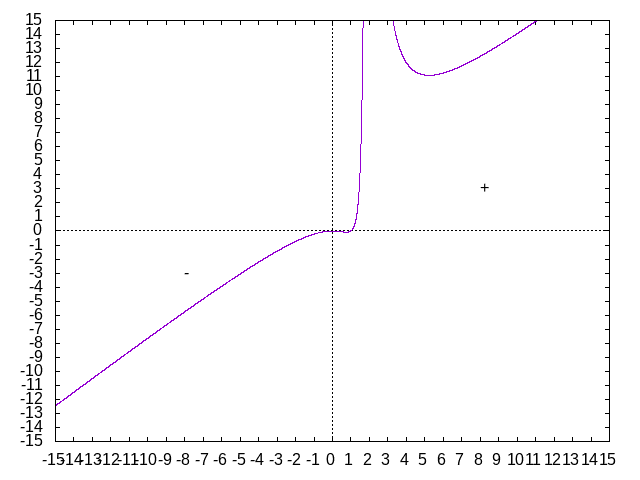
\includegraphics[scale=0.6]{funkcja2}
	\end{center}

	
\end{document}